\chapter{Background}%
\label{ch:background}

\newthought{In this chapter}, we introduce the minimally necessary background concepts our work is building upon. Our work marries two fields of research: on the one side generative, graphical models. With those one tries to model the data distribution of an observed variable by inducing dependencies of latent (unobserved) variables generating the observed variables. Modeling those dependencies, the meaningful latent variables allow us to build an intuitive generative story for the probabilistic model of the observed data. On the other hand, we introduce the recent body of work on how to practically model sound signals, in particular how this compares differently to modeling images.

First, we introduce the concept of deep latent-variable models, which important classes of models exist and how to train them. Second, we will shortly draw up the difficulties of modeling sound and which recent solutions exist and how they differ.

\section{Deep Latent-Variable Models}%
\label{sec:dlvm}
In this section, we introduce the idea of latent variable and the idea of finding models of data using those latent variables. Further, we discuss what practical ways are currently successful in estimating the model parameters and how they are trained.

For our process, we have observations from the data space \({\x}\∈\D\) for which there exists an unknown data probability distribution \(p^*(\D)\). We collect a data set \(\{\x_1\…\x_N\}\) with \(N\) samples. Further we introduce an approximate model with the density\footnote{We write density and distribution interchangeably to denote a probability function.} \(p_{\B{\θ}}(\D)\) and model parameters \(\B{\θ}\). Learning or modeling means finding the values for \(\B{\θ}\) which will give the closest approximation of the true underlying process:

\begin{equation}
    p_{\B{\θ}}(\D) \approx p^*(\D)
\end{equation}

The model \(p_{\B{\θ}}\) has to be complex enough to be able to fit the data density while little enough parameters to be learned. Every choice for the form of the model will \I{induce} biases\footnote{called \I{inductive biases}} about what density we can model, even before we maximize a learning objective using the parameters \(\B{\θ}\).

In the following described models we assume the sampled data points \(\x\) to be drawn from \(\D\) \I{independent and identically distributed}\footnote{meaning the sample of one datum does not depend on the other data points and we all draw them the same way}. Therefore we can write the data log-likelihood as:

\begin{equation}
    \log p_{\B{\θ}}(\D)
    = \Σ_{\x\∈\D} \log p_{\B{\θ}}(\x)
\end{equation}

The maximum likelihood estimation of our model parameters maximizes this objective.

To form a latent-variable model we introduce a \I{latent variable}\footnote{Latent variables are part of the directed graphical model but not observed.}. This latent variable can be any random variable underlying the generation of a data sample in \(\D\). For example, if we look at the generative story of a sound sample, a latent variable could be the sound source (the \I{instrument}). One can directly model the distribution of all musical notes played by all possible instruments. But we could also introduce the instrument as an underlying latent variable \(\z\), which would then lead to one distribution over this categorical variable and separate conditional densities of the sounds of each instrument. One of them then modeling the distribution of sounds made by a harp, for example.

Now the data likelihood is the marginal density of the joint latent density. With one latent variable we get:

\begin{equation}
    p_{\B{\θ}}(\x) = \∫ p_{\B{\θ}}(\x,\z) d\z
\end{equation}

Typically we introduce a factorization of the joint. The most common one and also the one from our previous example is:

\begin{equation}
    p_{\B{\θ}}(\x) = \∫ p_{\B{\θ}}(\x|\z)p(\z) d\z
    \label{eq:factorized_data_likelihood}
\end{equation}

\begin{marginfigure}%
    \begin{tikzpicture}
    \node[obs]                (x) {\(\x\)};
    \node[latent, left=of x]  (z) {\(\z\)};

    \edge {z} {x} ; %

    \plate {xz} {(x)(z)} {\(N\)} ;
\end{tikzpicture}

    \caption{The graphical model with a introduced latent variable \(\z\). Observed variables are shaded.}
    \label{fig:graphical_model}
\end{marginfigure}

This corresponds to the graphical model in which \(\z\) is generative parent node of the observed \(\x\), see~\cref{fig:graphical_model}. The density \(p(\z)\) is called the \I{prior distribution}.

If the latent is small, discrete, it might be possible to directly marginalize over it. If for example, \(\z\) is a discrete random variable and the conditional \(p_{\B{\θ}}(\x|\z)\) is a Gaussian distribution than the data model density \(p_{\B{\θ}}(\x)\) becomes a mixture-of-Gaussians, which we can directly estimate by maximum likelihood estimation of the data likelihood.

For more complicated models the data likelihood \(p_{\B{\θ}}(\x)\) as well as the model posterior \(p_{\B{\θ}}(\z|\x)\) are intractable because of the integration over the latent \(\z\) in \cref{eq:factorized_data_likelihood}.

To formalize the search for an intractable posterior into a tractable optimization problem we can follow the \I{variational principle}~\cite{jordanIntroduction1999} which introduces an approximate posterior distribution \(q_{\B{\φ}}(\z|\x)\), also called the \I{inference model}. Again the choice of the model here carries inductive biases, as such that even in asymptotic expectation we can not obtain the true posterior.

Following the derivation in~\textcite{kingmaIntroduction2019} we introduce the inference model into the data likelihood~\footnote{The first step is valid as \(q_{\B{\θ}}\) is a valid density function and thus integrates to one.}:

\begin{align}
    \log p_{\B{\θ}}(\x)
    &= \E_{q_{\B{\θ}}(\z|\x)} \left[ \log p_{\B{\θ}}(\x) \right]\\
    &= \E_{q_{\B{\θ}}(\z|\x)}
        \left[\log
        \÷{p_{\B{\θ}}(\x, \z)}
          {p_{\B{\θ}}(\z|\x)}
        \right]\\
    &= \E_{q_{\B{\θ}}(\z|\x)}
        \left[\log
        \÷{p_{\B{\θ}}(\x, \z)}
          {q_{\B{\φ}}(\z|\x)}
        \÷{q_{\B{\φ}}(\z|\x)}
          {p_{\B{\θ}}(\z|\x)}
        \right]\\
    &= \E_{q_{\B{\θ}}(\z|\x)}
        \left[\log
        \÷{p_{\B{\θ}}(\x, \z)}
          {q_{\B{\φ}}(\z|\x)}
        \right]
    +  \E_{q_{\B{\θ}}(\z|\x)}
        \left[\log
        \÷{q_{\B{\φ}}(\z|\x)}
          {p_{\B{\θ}}(\z|\x)}
        \right]\\
    &= \E_{q_{\B{\θ}}(\z|\x)}
        \left[\log
        \÷{p_{\B{\θ}}(\x, \z)}
            {q_{\B{\φ}}(\z|\x)}
        \right]
    +  \KL[q_{\B{\φ}}(\z|\x) \|
           p_{\B{\θ}}(\z|\x)  ]
\end{align}

Note that we separated the likelihood into two parts. The second part is the (positive) Kullback-Leibler divergence of the approximate posterior from the true intractable posterior. This unknown divergence states the `correctness' of our approximation~\footnote{More specifically the divergence marries two errors of our approximate model. First, it gives the error of our posterior estimation from the true posterior, by definition of divergence. Second, it specifies the error of our complete model likelihood from the marginal likelihood. This is called the \I{tightness} of the bound.}.

Therefore the first term becomes a lower  bound for the likelihood of the model. Also called the \I{variational free energy} or \I{evidence lower bound} (ELBO):

\begin{align}
    \elbo_{\B{\θ}, \B{\φ}}(\x)
    &= \E_{q_{\B{\θ}}(\z|\x)}
        \left[\log
        \÷{p_{\B{\θ}}(\x, \z)}
          {q_{\B{\φ}}(\z|\x)}
        \right]
    \label{eq:elbo}
\end{align}

We can introduce the same factorization as in~\cref{eq:factorized_data_likelihood}:

\begin{align}
    \elbo_{\B{\θ}, \B{\φ}}(\x)
    &= \E_{q_{\B{\θ}}(\z|\x)}
        \left[\log
        \÷{p_{\B{\θ}}(\x|\z) p(\z)}
          {q_{\B{\φ}}(\z|\x)}
        \right]\\
    &= \E_{q_{\B{\θ}}(\z|\x)}
        \left[\log
        \÷{p(\z)}
          {q_{\B{\φ}}(\z|\x)}
        \right]
    + \E_{q_{\B{\θ}}(\z|\x)}
        \left[\log p_{\B{\θ}}(\x|\z)\right]\\
    &= -\KL[q_{\B{\φ}}(\z|\x)\|p(\z)]
    + \E_{q_{\B{\θ}}(\z|\x)}
        \left[\log p_{\B{\θ}}(\x|\z)\right]
    \label{eq:elbo_factorized}
\end{align}

Under this factorization, we separated the lower bound into two parts. First, the divergence of the approximate posterior from the latent prior distribution and second the data posterior likelihood from the latent~\footnote{This will later be the reconstruction error. How well can we return to the data density from latent space?}.

The optimization of the \(\elbo_{\B{\θ}, \B{\φ}}\) allows us to jointly optimize the parameter sets \(\B{\θ}\) and \(\B{\φ}\). The gradient with respect to \(\B{\θ}\) can be estimated with an unbiased Monte Carlo estimate using data samples~\footnote{\( \∇_{\B{\θ}} \elbo_{\B{\θ}, \B{\φ}} \approxeq \∇_{\B{\θ}} \log p_{\B{\θ}} (\x, \z) \)}. Though we can \I{not} do the same for the variational parameters \(\B{\φ}\), as the expectation of the ELBO is over the approximate posterior which depends on \(\B{\φ}\). By a change of variable of the latent variable we can make this gradient tractable, the so called \I{reparameterization trick}~\cite{kingmaAutoEncoding2014}. We express the \(z\sim q_{\B{\θ}}\) as an random sample from a unparametrized source of entropy \(\B{\ε}\) and a parametrized transformation:

\begin{equation}
    \z = f_{\B{\η}}(\B{\ε})
\end{equation}

For example for a Gaussian distribution we can express \(z\sim \N(\μ,\σ)\) as \(z = \μ + \σ\·\ε\) with \(\ε\sim \N(0,1)\) and \(\η = \{\μ,\σ\}\).

\subsection{The VAE framework}

The variational autoencoder (VAE)~\footnotemark[\value{footnote}]~\cite{rezendeStochastic2014} presents a generative model using the above-introduced modeling of the joint distribution between an observed and latent variable to model to the latent variable. The model is split into two parts the encoder network and the decoder network. The encoder network parametrizes the approximate posterior \(\aprxpost\) by computing the parameters \(\B{\η}\) of the latent distribution. The decoder maps samples \(\z\sim q_{\B{\θ}}\) back into the data space. The optimization of the parameters of the two networks \(\{\B{\φ}, \B{\θ}\}\) is done by maximizing the ELBO (\cref{eq:elbo_factorized}).

End-to-end learning is made possible with the reparameterization trick and the algorithm looks like:

\begin{algorithm}
    \caption{Training's procedure for a variational autoencoder}%
    \label{alg:vae}
    \begin{algorithmic}[1]
        \While{Training is not converged}
            \State \(\B{X} \sim \D\)\Comment{Sample random mini-batch}
            \State \(\η \gets \text{EncoderNN}(\B{X})\)
            \State \(\B{\ε} \sim p(\B{\ε})\)
            \State \(\z \gets f_{\B{\η}}(\B{\ε})\)
            \State \(\B{X}' \gets \text{DecoderNN}(\z)\)
        \EndWhile%
    \end{algorithmic}
\end{algorithm}

The \β-VAE~\cite{higginsBetaVAE2016} extends the VAE objective with an \(\β\) hyperparameter in front of the KL divergence. The value \(\β\) gives a constraint on the latent space, controlling the capacity of it. Adapting \(\β\) gives a trade-off between the reconstruction quality of the autoencoder and the simplicity of the latent representations\footnotemark[\value{footnote}]. Using such a constraint is similar to the use of the information bottleneck~\cite{burgessUnderstanding2018}.

\subsection{Flow based models}%
\label{subsec:flows}

The VAE and other related generative models, define the joint distribution between the latent and the observed variables. Another way of attacking the problem is a \I{change of variable} where we learn a function that changes the observed variable into the latent one, also known as  \I{normalizing} flows~\cite{tabakFamily2013}. A normalizing flow is a function \(f: \mathcal{X}\to \mathcal{Z}\) that maps the input density to a fixed, prescribed density \(p(\ε) = p(f(\x))\), in that normalizing the density~\footnote{The extreme of this idea is an infinitesimal, continuous-time flow with a velocity field.}. With \(f(\·)\) we can then integrate over \x  and \z with the each other:

\begin{align}
    &\∫_{\mathcal{Z}} p(\z) d\z = \∫_{\mathcal{X}} p(f(\x)) {\Big|\pf{f}{\x}\Big|} d\x\\
     &= \∫_{\mathcal{X}} p(\x) dx = \∫_{\mathcal{Z}} p(f^{-1}(\z)) \Big|\pf{f^{-1}}{\z}\Big| d\z
\end{align}

The terms \({\Big|\pf{f}{\x}\Big|}\) and \({\Big|\pf{f^{-1}}{\z}\Big|}\) adapt the volumes under the measure. They are the determinant of the Jacobian matrix of the function \(f\).

With this setup, we can choose a fixed distribution \(p_{\z}(\z)\) and can optimize the model only in terms of the transformation into this auxiliary variable:

\begin{equation}
    \B{\θ}^* = \argmax_{\B{\θ}} \Σ_n^N \log p_{\z}(f_{\B{\θ}}(\x_n)) + \log {\Big|\pf{f_{\B{\θ}}}{\x_n}\Big|}
\end{equation}

For a finite normalizing flow, we consider a chain of invertible, smooth mappings making the composite \(f\). The difficulty arises, from the condition, that we need to be able to compute the log-determinant of each flow function's Jacobian. Careful design of the flow functions is necessary to assure a cheap computation of the log-determinant while allowing for complex models to be learned.

The first deep model to successfully do so is NICE~\cite{dinhNICE2015} which introduced coupling layers to parametrize the flow steps. In the coupling layer the input \x is split in two equally sized parts \(\x_a\) and \(\x_b\). Then the first split is transformed by translation factors computed from the second split:

\begin{align}
    \B{y}_a &= \x_a + t(\x_b)\\
    \B{y}_b &= \x_b
\end{align}

The translation function \(t(\·)\) can be implemented as any complex operation. These additive coupling layers are volume-preserving and as such have their Jacobian's determinant is 1.

RealNVP~\cite{dinhDensity2017} builds on top of NICE creating a non-volume preserving, normalizing flow. By extending the coupling layers to affine transformations:

\begin{align}
    \B{y}_a &= \exp{(s(\x_b))} \odot \x_a + t(\x_b)\\
    \B{y}_b &= \x_b
\end{align}

Again the scale \(s(\·)\) and translation \(t(\·)\) functions can be implemented with complex functions such as deep neural networks. As these transformations are non-volume preserving the Jacobian's determinant needs to be computed. Because of the design of the coupling layers the Jacobian reduces to:

\begin{equation}
    \pf{\B{y}}{\x^T} = \bM{\1 & 0 \\ \pf{\B{y}_a}{\x^T_b} & \diag{\left(\exp{(s(\x_b))}\right)}}
\end{equation}

Which means the efficiently compute the determinant with:

\begin{equation}
    \Big|\pf{f}{\x}\Big| = \exp{\left[\Σ_i {s(\x_b)}_i\right]}
\end{equation}

The authors provide multiple ideas on how to split an input tensor with spacial masking using repeating checkerboard patterns. Further, it is also important that the masking of the two splits is inverted/changed throughout a combination of multiple coupling layers so that the split into transformer and transformed part is not fixed.

Glow~\cite{kingmaGlow2018} extended the RealNVP by introducing invertible 1\×1-convolutions. Instead of having fixed masks and permutations for the computations of the affine parameters in the coupling layer, Glow learns a rotation matrix which mixes the channels. After mixing the input can always be split into the same two parts for the affine transformation. Further, the authors showed that training can be helped by initializing the last layer of each affine parameter network with zeros. This ensures that at the beginning without weight update each coupling layer behaves as an identity.

\section{Langevin dynamics}%
\label{sec:langevin}
Another topic we are gonna touch on in our research are sampling techniques, more specifically Langevin dynamics.

Let's take a step back and look at the typical procedure in a stochastic optimization~\cite{robbinsStochastic1951} process. Let \(\B{\θ}\) denote a parameter vector for which we want to find a maximum-a-posteriori solution given the data \(\B{X} = \{\x_i\}_i^N\).  In stochastic optimization, we update the parameters \(\B{\θ}\) with the gradient of the posterior using a subset of samples from our data set:

\begin{align}
    \Δ\B{\θ}_t &= \÷{\ε_t}{2} \{(\∇\log{p(\B{\θ}_t)}) + \÷{N}{n}\Σ_{i=1}^n \∇\log{p(x_{ti} | \B{\θ}_t)}\}
\end{align}

With a prior distribution for the parameters \(p(\B{\θ})\). By taking the gradient of the posterior only under a subset of the data will give us a noisy estimate of the real gradient, but is computationally cheaper. The idea is, that the noise of the noisy gradients smoothes out while sampling different subsets. When using a decaying step size \(\ε_t\) the stochastic optimization is guaranteed to converge to a local maximum. The problem with this approach is though, that we are not considering any uncertainty of the parameter updates.

To remedy this risk \textcite{wellingBayesian2011} introduced the ideas of Langevin dynamics~\cite{nealMCMC2012} into the update step to form \I{Stochastic Gradient Langevin Dynamics} (SGLD). The idea is that we introduce Gaussian noise in every update step of the optimization where the noise is scaled by the decreasing learning rate \(\ε_t\):

\begin{align}
    \Δ\B{\θ}_t &= \÷{\ε}{2}\{( \∇\log{p(\B{\θ}_t)} + \÷{N}{n}\Σ_{i=1}^N \∇\log{p(x_i | \B{\θ}_i)} )\} + \η_t\\
    \η_t &\sim \N(0, \ε)
\end{align}

Formally we want to take the updated proposal distribution and form a Markov chain Monte Carlo (MCMC) with Metropolis-Hastings to accept or reject the proposal. Because we are scaling the injected noise with decaying learning rate Welling \& Teh\footnotemark[\decrvalue{footnote}{1}] showed that the validation of the proposal distribution can be ignored. The rejection rate goes to zero.

Thus SGLD gives a computationally cheap method to do stochastic weight updates while capturing the uncertainty of the parameters.

\section{Modeling audio}%
\label{sec:audio}
Lastly, we introduce the difficulties and approaches to modeling audio or sound signals.

In the physical world, a sound signal is a density change of the carrier air over time. As such it is a one-dimensional temporal signal\footnote{Sound waves in gases are purely compressive, therefore they cannot be polarized which would introduce a higher complexity. In solids a sound signal can have polarization, think of an earthquake with shear and pressure components.}. Humans sound perception is \I{stereo} as we have two ears and sense the changes in pressure at two different points in space simultaneously.

\subsection{Representations of audio}%
\label{subsec:audio}
The simplest form of digitally representing a sound signal is recording the amplitude at fixed intervals at one or multiple points in space with a microphone. This method is called Pulse-Code modulation (PCM). It introduces two parameters which will bias the result of the record. First we have to pick a temporal frequency with which the pressure samples are taken, the so-called sample rate. The Nyquist-Shannon theorem~\cite{kotelnikovCarrying1933} tells us that if the highest frequency in the true signal is \(B\ \si{\Hz}\) than with a sample rate of \(2\· B\ \si{\Hz}\) we will capture the complete signal with all frequencies. At a lower sample rate, we might introduce aliasing effects. Second, we have to represent each amplitude sample as a digital value. Most commonly the sample is encoded into a \(\SI{8}{\bit}\) or \(\SI{16}{\bit}\) integer. The microphone has a range of air pressure which w.l.o.g.\ we set to \([-1, 1]\), where a value of 0 is no signal, 1 shows maximum compression and -1 maximum decompression of the carrier air.  The simplest form of encoding is Linear PCM. In Linear PCM, amplitudes are quantized on an evenly spaced grid over the possible value range. More advanced quantization include \(\μ\)-law encoding~\cite{Pulse1972} in which the quantization intervals are varied with the amplitude\footnote{The actual formula for calculating the \(\μ\)-law quantization is: \[\t{\μ -law}(x) = \sgn{(x)} \· \÷{\ln{(1 + \μ |x|)}}{\ln{(1 + \μ)}}\]}. As the human perception of loudness is logarithmic this encoding also quantizes the amplitude values on a logarithmic response curve. Simply speaking the lower amplitudes will be quantized on a finer grid than higher amplitudes. This makes it possible to achieve a higher signal-to-noise ratio at smaller encoding sizes for sound signals.

As an example, if encoding a sound signal with \(\SI{8}{\kHz}\) \(\SI{16}{\bit}\) Linear PCM we sample an amplitude value every \(\÷{1}{8000} \si{\s}\) and quantize those into \(2^{16} = 65536\) bins. A sample with 100 values is only \(\SI{12.5}{\ms}\) long!

A standard full piano with 88 keys tuned to \(\SI{440}{\Hz}\) at the \(\t{A}_4\)\cite{iso/tc43acousticsISO1975} has a frequency range of \([\SI{27.5}{\Hz}, \SI{4186}{\Hz}]\) from the \(\t{A}_0\) to the \(\t{C}_8\), respectively. Therefore just for the recording of a standard piano we need a sampling rate of more than \(\SI{8}{\kHz}\). Beyond the piano, many instruments exhibit even larger frequency content which leads to the conclusion that not just for recording but also for our goal of modeling musical sounds a reasonably high sampling rate is crucial.

Looking at the temporal scales of musical information, on the small end we have the modeling of pitch as discussed before which happens at scales of \([10^{-1}\,\si{\ms}, 10^2\,\si{\ms}]\) over single notes happening at scales of \([10^2\,\si{\ms}, 10^3\,\si{\ms}]\) to the structure of melodies and full songs happening at \([10^4\,\si{ms}, 10^6\,\si{\ms}]\). The modeling of music happens over 7 magnitudes of time! In \cref{sec:raw_audio} we will present common solutions to this difficulty.

\subsection{Spectrograms}
Commonly used alternative representations of signals in sound processing are spectrograms. A spectrogram is a mapping of the time-domain wave signal into a frequency domain. With a Fourier transform~\cite{fourierTheorie1822} it is possible to represent any function as an (at worst) infinite sum of harmonics, or trigonometrical signals. The Fourier transform is a complex-valued function where the absolute value gives the amount a given cosine with that frequency is present in the signal.

\begin{equation}
    \hat{f}(\ν) = \∫_{-\infty}^{\infty} f(x) e^{-2\π i x \ν}dx
\end{equation}

\begin{marginfigure}
    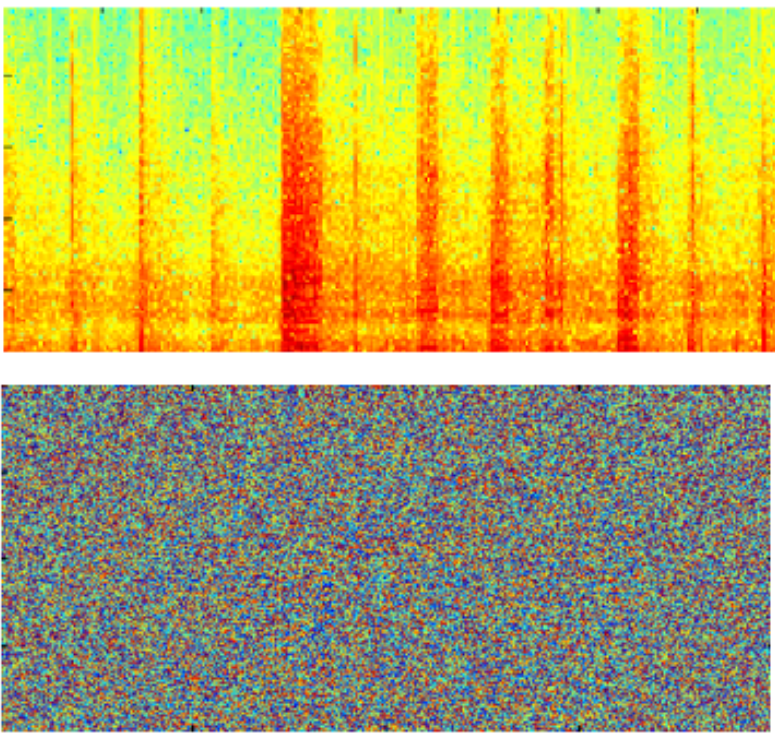
\includegraphics[width=2in]{phase_spec.png}%
    \label{fig:phase_spec}%
    \caption{The STFT magnitude and the corresponding phases for each sinusoidal.}
\end{marginfigure}

Where \(f(x)\) is the original time-domain signal and \(\ν\) is a frequency of interest.

The idea for signal/music processing is that with a transformation into frequency space we can handcraft a response feature similar to how the hairs in the cochleae of the human inner ear react to different frequencies of the pressure wave. A Fourier transform gives the frequency content of the whole signal but we are interested in the change of frequencies present in a given signal over time. For this, the most common transformation is the Discrete Short-time Fourier transform (STFT)~\cite{grochenigFoundations2001}. For the STFT the Fourier transformation is applied to overlapping windows sliding over the signal. As our signal is a discrete sample of the true signal, a discrete implementation is needed.

An unmodified Fourier transform is linear in frequency. Humans do not perceive changing frequency (pitch) in this way. First, there is an individual lower and upper bound to human perception of frequency. Second, changing frequencies are not perceived linearly in their pitch\footnote{Pitch is the human perception of a sound being \I{high} or \I{low}.}. Pitch perception is sublinear\cite{stevensScale1937}. To allow a spectrogram to reflect this perceived importance  Mel-scales\footnote{Mel(ody)} are commonly applied. The Mel scale compresses the frequency range with a logarithm which parameters are determined from perceptional experiments. A common transformation is~\cite{douglasSpeech2000}:

\begin{equation}
    \hat{\ν} = 2595 \· \log_{10}\left( 1 + \÷{\ν}{700} \right)
\end{equation}

When using a spectrogram for signal processing we have to choose the form of the spectrogram being used. First, most commonly one would use the magnitude of the complex spectrogram to access the actual frequency contents. By that, we are disregarding the phase of these harmonics though. Trying to model the phase separately to the frequency is futile, see~\cref{fig:phase_spec}. Alternatively one can use an approximate vocoder to reverse the destructive reduction of the complex spectrogram (e.g.~\cite{chandnaVocoder2019a}) or directly model the complex spectrogram which has been used for some tasks with success~\cite{tanComplex2019,liuSupervised2019,lerouxPhasebook2019}. Many recent deep learning approaches to sound processing model a time-frequency map which is used to filter the original spectrogram~\cite{chandnaMonoaural2017,andreasjanssonSinging2017}. As such the phase from the input signal is used in the resulting output signal. While often these approximate approaches are successful in practice the usage of magnitude spectrograms introduces undefined limits into, which might inhibit performance~\cite{lluisEndtoend2019}.

\subsection{Modeling raw audio}%
\label{sec:raw_audio}
Deep learning models as used for image applications are unsuitable for raw audio signals (signals in \I{time-domain}). Digital audio is sampled at high sample rates, commonly 16kHz up to 44kHz. The features of interest lie at scales of strongly different magnitudes. Recognizing the local-structure of a signal, like frequency and timbre, might require features at short intervals (\(\approx\) tens of milliseconds) but modeling of speech or music features happens at the scale of seconds to minutes. As such a generative model for this domain has to model at these different scales.

\begin{figure}
    \begin{tikzpicture}[scale=0.6, every node/.style={scale=0.6}]
    \begin{scope}
        \draw[xstep=18cm, dashed] (1,1) grid (18,5);

        \begin{scope}[xshift=0.5cm,yshift=0cm,canvas is xz plane at y=1]
            \draw[fill=blue,draw=none,fill opacity=.2]
                (0,0) sin (1,1)  cos (2,0)  sin (3,-1)  cos (4,0)
                      sin (5,1)  cos (6,0)  sin (7,-1)  cos (8,0)
                      sin (9,1)  cos (10,0) sin (11,-1) cos (12,0)
                      sin (13,1) cos (14,0) sin (15,-1) cos (16,0)
                      sin (17,1) cos (18,0);
        \end{scope}

        \foreach \x in {1,...,18} {
            \node[inner sep=.15cm, fill=blue] () at (\x,1) {};
            \node[inner sep=.15cm, fill=orange] () at (\x,5) {};
        }

        \foreach \x in {1,...,18} {
            \foreach \y in {2,...,4} {
                \node[draw=black,fill=white] (thisNode) at (\x,\y) {};
            }
        }

        \draw[decorate,decoration={brace,amplitude=4pt}]
        (0.75,1.8) -- (0.75,4.2) node [black,midway,xshift=-.4cm, rotate=90] {\small
        hidden layers};

        \draw[->] (1,0.4) -- (18.5,0.4) node[right] {time \(t\)};
    \end{scope}

    \begin{scope}[shift={(18,5)}]
        \graph [grow down, branch left=1cm, empty nodes, nodes={rectangle}, edges={draw,black}] {
            "" -- {
                "" -- {
                    "" -- { "" -- {"",""}, "" -- {"",""}},
                    "" -- { "" -- {"",""}, "" -- {"",""}}
                },
                "" -- {
                    "" -- { "" -- {"",""}, "" -- {"",""}},
                    "" -- { "" -- {"",""}, "" -- {"",""}}
                }
            }
        };
    \end{scope}
\end{tikzpicture}

    \caption[][-2em]{An example of how dilated convolutions are used in the WaveNet. We see three hidden layers with each a kernel size of two. By using the dilations the prediction of the new output element has a receptive field of 18. This convolution is \I{causal} as the prediction depends only on previous input values. Causality is enforced through asymmetric padding.}%
    \label{fig:wavenet}
\end{figure}

The \B{WaveNet}~\cite{vandenoordWaveNet2016} introduced an autoregressive generative model for raw audio. It is build upon the similar PixelCNN~\cite[\protect\label{pixelcnn}]{vandenoordConditional2016} but adapted for the audio domain.  The WaveNet accomplishes this by using dilated causal convolutions.
Using a stack of dilated convolutions increases the receptive field of the deep features without increasing the computational complexity, see~\cref{fig:wavenet}. Further, the convolutions are gated and the output is constructed from skip connections. For the structure of a hidden layer refer to \cref{fig:wavenet_layer}. A gated feature, as known from the LSTM~\cite{hochreiterLong1997a}, computes two outputs: one put through an sigmoid \(\σ(\·)\) activation and one through an \(\tanh(\·)\) activation. The idea being that the sigmoid (with an output range of \([0, 1]\)) regulates the amount of information, thereby gating it, while the \(\tanh\) (with a range of \([-1,1]\)) gives the magnitude of the feature.
\begin{figure}
    \centering
    \begin{tikzpicture}
    \matrix[]
    {
        & & \node (g)  {g}; &
        \node (gs) {\(\σ\)}; & & & & &\\

        \node (featold) {}; &
        \node (dilate) {dilate}; & & &
        \node (times)  {\(\odot\)}; & &
        \node (chfeat) {\(1\× 1\)}; &
        \node (plfeat) {+}; &
        \node (featnew) {};\\

        & & \node (f) {f}; &
        \node (ft)  {\(\tanh\)}; & &
        \node (chskip) {\(1\× 1\)}; & & &\\

        \node (skipold) {}; & & & & &
        \node (plskip) {+}; & & &
        \node (skipnew) {};\\
    };
    \begin{scope}[every path/.style={draw, ->}]
        \path (featold) -- (dilate);
        \path (dilate) |- (g);
        \path (dilate) |- (f);
        \path (g) -- (gs);
        \path (f) -- (ft);
        \path (gs) -| (times);
        \path (ft) -| (times);
        \path (times) -- (chfeat);
        \path (chfeat) -- (plfeat) -- (featnew);
        \path (times) -| (chskip);
        \path (chskip) -- (plskip);

        \path (dilate) |- (1,1) -| (plfeat);

        \path (skipold) -- node [near start] {skip} (plskip) -- (skipnew);
    \end{scope}
\end{tikzpicture}
%
    \caption[][-2em]{A hidden layer as in the WaveNet. We have the four convolutions, with the filter \(f^*\) and gate \(g^*\) being dialted and the two channel mixing filters. Information flows along the skip connection that gets added up and the residual which receives the original input.}%
    \label{fig:wavenet_layer}%
\end{figure}
The output of the WaveNet is the sum of outflowing skip connections added after each (gated) hidden convolution. This helps fusing information from multiple time-scales (\I{low-level} to \I{high-level}) and makes training easier~\cite{szegedyGoing2014}. The original authors tested the model on multiple audio generation tasks. They used a \μ-law encoding~\cite{Pulse1972} which discretizes the range \([-1, 1]\) to allow a set of \μ targets and a multi-class cross-entropy training objective. While being quite unnatural this is done to avoid making any assumptions about the target distribution. Sound generation with a WaveNet is slow as the autoregressiveness requires the generation value by value. The original WaveNet setting is generating waveforms, by giving the previously generated values as the input and conditioning the process on target classes, \(p(x_t|x_{1:t},c_t)\). Therefore the generation has to happen value-by-value (autoregressive). This can be alleviated by keeping intermediate hidden activations cached~\cite{paineFast2016}. The WaveNet can be conditioned by adding the weighted conditionals in the gate and feature activations of the gated convolutions~\cite{vandenoordConditional2016}.

One of the first latent generative models to employ a WaveNet is NSynth~\cite{kalchbrennerEfficient2018}. They construct an autoencoder in which both encoder and decoder are WaveNet-like. The \I{non-causal temporal encoder} uses a stack of dilated residual non-causal convolutions. The convolutions are not gated and no skip-connections are used. The decoder is a WaveNet taking the original input chunk as an input and predicts the next value of the sound sample, while being conditioned on the latent variable. The authors use this model to learn latent temporal codes from a new large set of notes played by natural and synthesized instruments. The latent of the VAE is conditioned on the pitch of these notes. While the model is difficult to train, they show great improvement of the WaveNet-based VAE compared to a spectral-based autoencoder.

\textcite{chorowskiUnsupervised2019} presents a WaveNet-based VAE.\@They are learning speech representations, unsupervised. The encoder is a residual convolutional network and takes a Mel-scaled spectrogram of the signal as its input. As the bottleneck they found a VQ codebook~\cite{vandenoordNeural2017} to be most successful. The decoder is an autoregressive WaveNet conditioned on the latent features. While the input to the encoder is a spectrogram the decoder reconstructs the waveform of the signal.

Multiple works have combined the WaveNet architecture with the \sref{subsec:flows}. In WaveGlow~\cite{prengerWaveGlow2018} the authors parametrize the affine coupling layers of a Glow model with WaveNets and keeping the rest of the architecture similar to the original Glow with the \(1\× 1\)-convolutions. The authors apply this model to the task of speech synthesis where Mel-spectrograms are generated from the true audio. Then all WaveNets in the coupling layers are conditioned on the spectrogram. The model therefore learns the waveform generation task given spectral features (a vocoder). WaveGlow is outperforming similar approaches and the needlessness of autoregressiveness gives the model fast performance.

The FloWaveNet~\textcite{kimFloWaveNet2019} is a similar model building a flow from WaveNets. As in WaveGlow, the affine coupling layers are parametrized by WaveNets. The model is more similar to the RealNVP in that the flexibility of the flows is achieved by flipping the channels of the data after a flow operation instead of learning a channel mixing convolution. Each coupling flow layer is preceded by an Activation Normalizing operation as in Glow.
